
\documentclass[a4paper,12pt]{article} % тип документа

% report, book

% Рисунки
\usepackage{graphicx}
\usepackage{wrapfig}

\usepackage{hyperref}
\usepackage[rgb]{xcolor}



%  Русский язык

\usepackage[T2A]{fontenc}			% кодировка
\usepackage[utf8]{inputenc}			% кодировка исходного текста
\usepackage[english,russian]{babel}	% локализация и переносы


% Математика
\usepackage{amsmath,amsfonts,amssymb,amsthm,mathtools} 


\usepackage{wasysym}

%Заговолок
\author{Сафиуллин Роберт	}
\title{Лабораторная работа 1.3.3}

\title{Определение вязкости воздуха по скорости течения через тонкие
трубки}





\begin{document} % начало документа

\maketitle


\newpage
\section{Цель работы:}
1)  Экспериментально выявить участок сформированного течения, определить режимы ламинарного и турбулентного течения; определить число Рейнольдса.\\
\section{В работе используются:}
Металлические трубки, укрепленные на горизонтальной подставке; газовый счетчик; микроманометр типа ММН; стеклянная U-образная трубка; секундомер.
 \section{Описание работы}
 Рассмотрим движение вязкой жидкости или газа по трубке круглого сечения. При малых скоростях потока движение оказывается ламинарным (слоистым), скорости частиц меняются по радиусу и направлены вдоль оси трубки. С увеличением скорости потока движение
становится турбулентным, и слои перемешиваются. При турбулентном движении скорость в каждой точке быстро меняет величину и направление, сохраняется только средняя величина скорости.

Характер движения газа (или жидкости) в трубке определяется безразмерным числом Рейнольдса: $$Re=\frac{vrp}{\eta}$$

В гладких трубах круглого сечения переход от ламинарного движения к турбулентному происходит при $Re \approx 1000$.

При ламинарном течении объем газа V, протекающий за время t по трубе длиной l (называемый расходом), определяется формулой Пуазейля: $$Q_V=\frac{\pi r^4}{8l\eta}(P_1-P_2)$$
При	втекании	газа	в	
трубку	из большого резервуара скорости слоев вначале постоянны по всему сечению (рис. 1). 
 По мере продвижения  газа по	трубке	
картина распределения скоростей меняется, так как сила трения о стенку тормозит прилежащие к ней слои. Характерное для ламинарного	
течения параболическое распределение скоростей устанавливается на	
некотором расстоянии a от входа в трубку, которое зависит от радиуса трубки r и числа Рейнольдса по формуле: $$a\approx0,2r*Re$$.\\

\section{Ход работы}

1)
В работе используются две узкие трубки (1 и 2) с диаметрами:

$d_1$ = 3.85 $\pm$ 0.05мм\\

$d_2$ = 5.85 $\pm$ 0.05мм

Оценим расстояние, на котором происходит формирование потока при ламинарном течении:

$a_1$$\approx0,2r*Re=0,2*3,85/2*10^{-2}*1000\approx$38.5 $\pm$ 0.5см\\

$a_2$$\approx0,2r*Re=0,2*5,85/2*10^{-2}*1000\approx$58.5 $\pm$ 0.5см

Давление, измеряемое микроманометром, определяется по формуле:
$$P=0.2*809*N*9,80665$$
2) Возьмем зависимость $\triangle$P(Q). Используя секундомер и газовый счетчик найдем расход воздуха по формуле: Q=$\triangle$P/$\triangle$t

Результаты запишем в таблицу:

\begin{tabular}{|c|c|c|c|c|c|}
\hline 
N$\pm0.5$, дел & 206 & 67 & 86 & 52 & 107 \\ 
\hline 
P$\pm0.8$, Па & 403.76 & 106,238 & 136.37 & 82.45 & 169.66 \\ 
\hline 
Q$\pm0.05$, л/с & 0.14 & 0.085 & 0.98 & 0.07 & 0.101 \\ 
\hline 
\end{tabular} 
\newpage

Используя ее, построим график $\triangle$P(Q)

\begin{center}
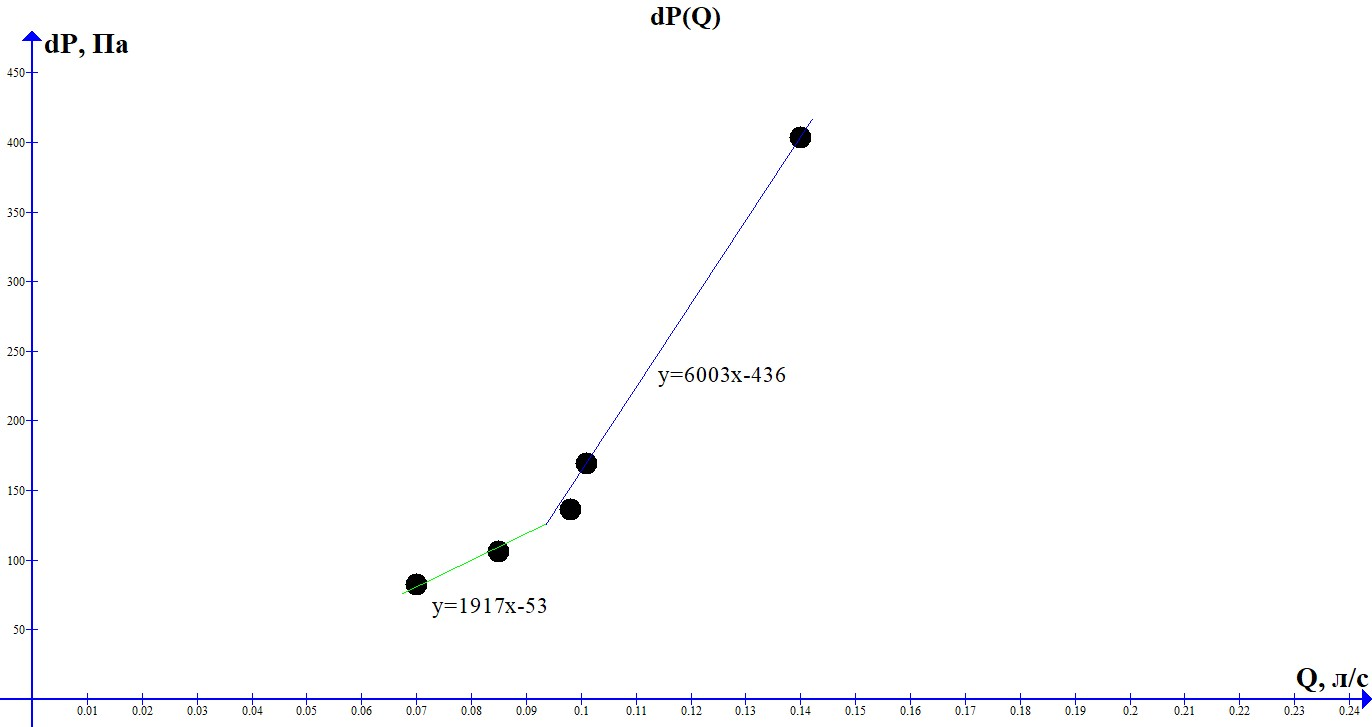
\includegraphics[scale=0.33]{1331}
\end{center}


С помощью коэффицента наклона k графика посчитаем вязкость воздуха из формулы:

N=$\eta$*$\frac{8l}{\pi*r^{4}*0.2*9.8*8.80665*Q}$

$\eta = \frac{\pi r^4  k}{8l}$=2.06$\pm0.18$ *$10^{-5}$ Па*c\
Табличное значение: 1.812*$10^{-5}$ Па*c


Где длина участка на котором проводятся измерения:
l=50 cм \\

3) Найдем число Рейнольдса по формуле:  $Re=\frac{\rho v r}{\eta}$, используя, что

 $\rho=\frac{p_0 M}{R T_0}$
 
$v=\frac{Q}{\pi r^{2}}$

А также зная, что ламинарный режим переходит в турбулентный при значении Q=0.095 л/c

Re=893




















4) Исследуем распределение давления вдоль трубки путем последовательного подсоединения манометра ко всем ее выводам. результаты Запишем в таблицу:\\

\begin{tabular}{|c|c|c|c|c|c|}
\hline 
\multicolumn{6}{|c|}{1 трубка}\\ 
\hline 
\hline 
Участок & 3-4 & 2-4 & 2-5 & 1-4 & 1-5 \\ 
\hline 
N, дел & 31 & 52 & 88 & 77 & 113 \\ 
\hline 
\end{tabular} 
\begin{tabular}{|c|c|c|c|c|c|c|}
\hline 
\multicolumn{7}{|c|}{2 трубка}\\ 
\hline 
\hline 
Участок & 1-5 & 1-4 & 1-3 & 2-4 & 2-5 & 3-5 \\ 
\hline 
N, дел & 103 & 75 & 53 & 44 & 70 & 50 \\ 
\hline 
\end{tabular} 

Переведем эти данные в зависимость P(l):  \\
\begin{tabular}{|c|c|c|c|c|}
\hline 
\multicolumn{5}{|c|}{1 трубка}\\ 
\hline 
\hline 
Участок & 1-2 & 1-3 & 1-4 & 1-5 \\ 
\hline 
l, cm & 11.4 & 41.4 & 81.4 & 131.4 \\ 
\hline 
P$\pm0.8$, Pa & 39.6 & 72.94 & 122 & 179.18 \\ 
\hline 
\end{tabular} 
\begin{tabular}{|c|c|c|c|c|}
\hline 
\multicolumn{5}{|c|}{2 трубка}\\ 
\hline 
\hline 
Участок & 1-2 & 1-3 & 1-4 & 1-5 \\ 
\hline 
l, cm & 11.4 & 41.4 & 81.4 & 131.4 \\ 
\hline 
P$\pm0.8$, Pa & 49.15 & 84 & 118.9 & 163.32 \\ 
\hline 
\end{tabular} \\ 

Используя их, построим график P(l)

\begin{center}
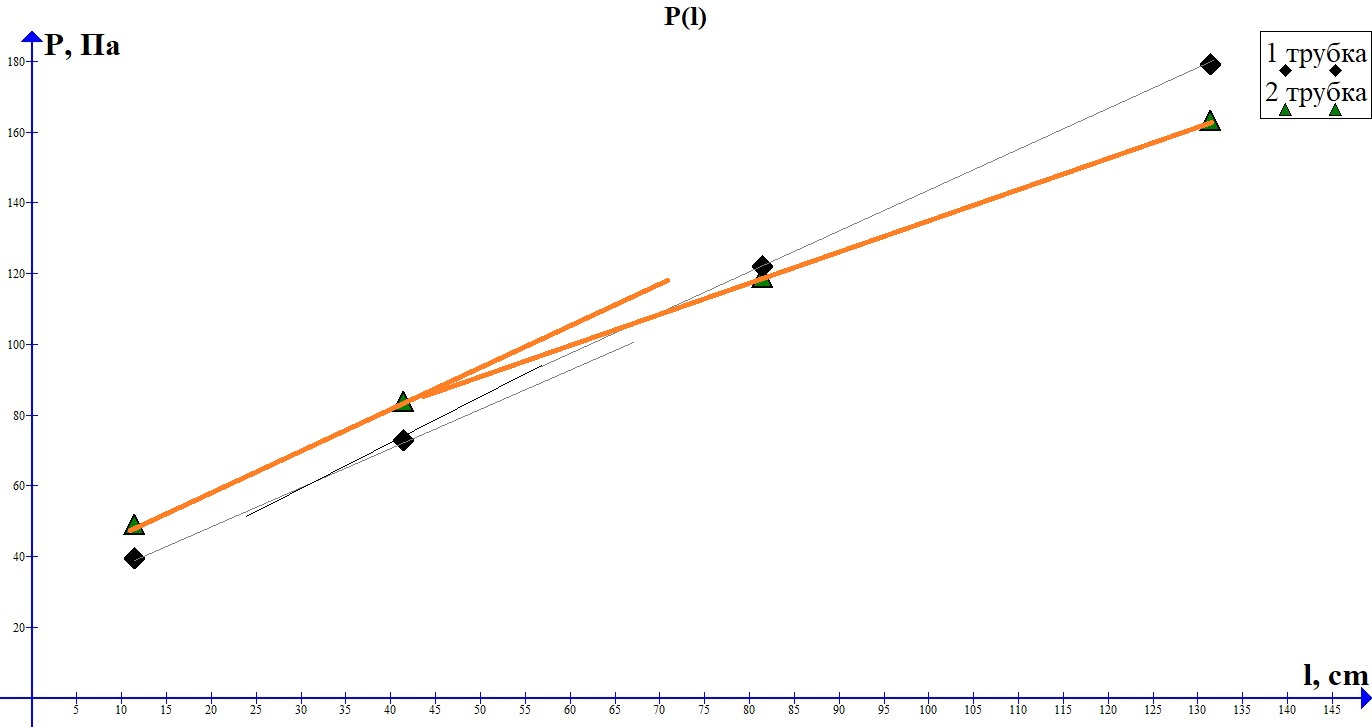
\includegraphics[scale=0.55]{1332}
\end{center}

Отсюда видно, что установление потока происходит на расстояниях 30 см для 1 трубки и 42 см для 2 трубки. И поэтому можно сделать вывод, что оценка, полученная формулой, является грубой.

5) Для обеих трубок на участках со сформированным течением в ламинарном режиме снимем зависимость Q(P) и обработаем ее по формуле 
$$\frac{8l\eta Q}{\pi(P_1-P_2)}=r^n$$
$$\ln(\frac{8l\eta Q}{\pi(P_1-P_2)})=n\ln r$$
$$\ln1=n\ln2$$

Pезультаты занесем в таблицу:

\begin{tabular}{|c|c|c|c|c|c|c|}
\hline 
• & \multicolumn{3}{|c|}{1 трубка} & \multicolumn{3}{|c|}{2 трубка} \\ 
\hline 
N$\pm0.5$, дел & 69 & 140 & 202 & 42 & 92 & 128 \\ 
\hline 
$\triangle$P$\pm0.8$, Pa & 109.4 & 222 & 320.3 & 66.6 & 145.88 & 203 \\ 
\hline 
Q$\pm0.05$, л/с & 0.083 & 0.125 & 0.132 & 0.166 & 0.25 & 0.29 \\ 
\hline 
Ln1 & -26.72 & -27 & -27.33 & -25.53 & -25.9 & -26.01 \\ 
\hline 
ln2  & \multicolumn{3}{|c|}{-6.25} & \multicolumn{3}{|c|}{-5.83} \\ 
\hline 
\end{tabular} 


И по ним построим график Ln1(Ln2):
\begin{center}
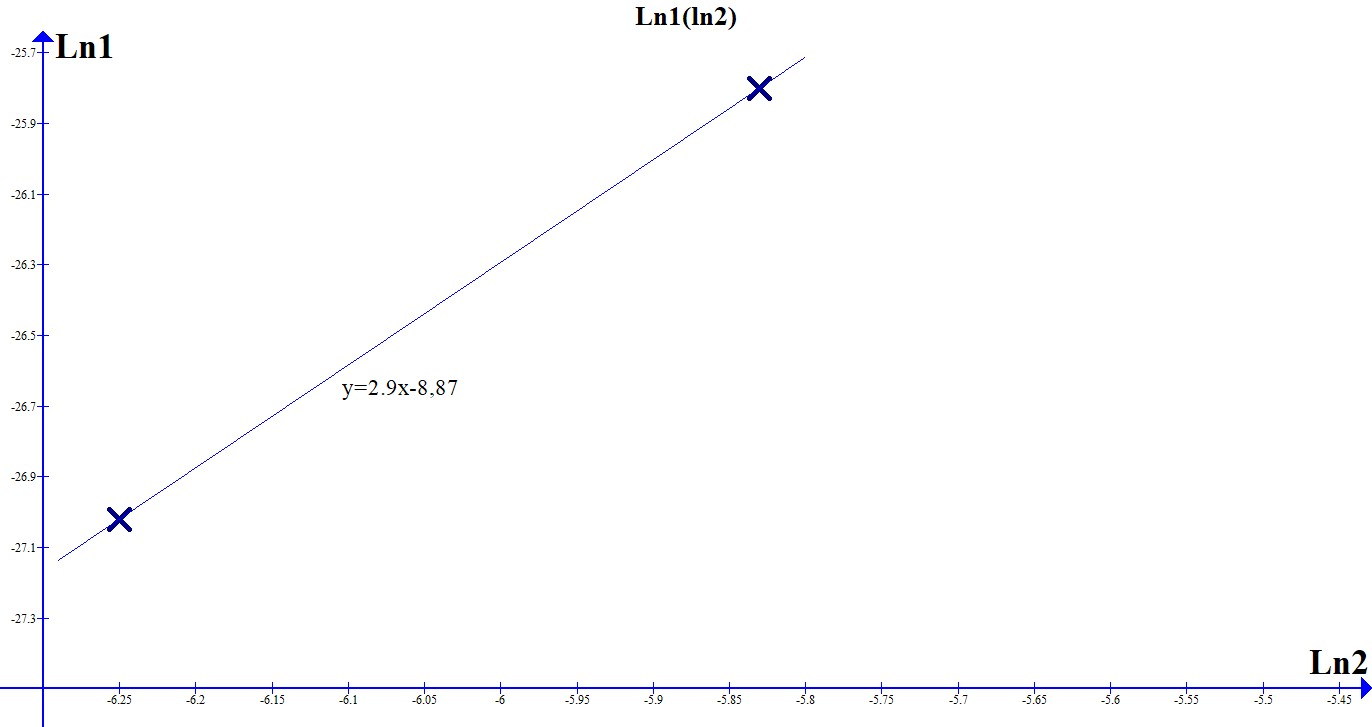
\includegraphics[scale=0.33]{1333}
\end{center}

Отсюда n=2.9$\pm$0.8, т.к. наибольший вклад в погрешность $\frac{ln1}{ln2}$ вносит $\sigma_P$=0.8.

Итого: табличные результаты взякости воздуха и показателя степени в формуле Пуазейля находятся в пределах погрешности проделанных измерений.





























\end{document} % конец документа